\section{Mathematical Background}
The purpose of this document is to provide the mathematical foundation to understand analytical network capacity analysis under spatial structures using point processes (PP).  To understand this analysis requires a significant amount of background understanding in point processes and how they have been used in the literature to model wireless network interference.  Using spatial geometry has significant advantages for interference modeling as it provides analytic tools for characterization.  Networks can be modeled over spatial distributions rather than single realizations.  This provides more generalized results, over any network configuration.  This does come at the cost of mathematical convenience.\par
%

We will first begin with an introduction to PP and how we relate them to the physical structure of the network.  Next we will introduce a mathematical description of the network interference through a concept called shot noise (SN), based on the original work of Schottkey in 1918\todo[size=\small, color=green!40]{Get citation}.  %\cite{}.
Then with SN based interference we will derive network wide performance metric and bounds.  Finally we will introduce medium access control (MAC), and the associated mathematically model in this PP framework. Slotted Aloha, CSMA, FDMA, and TDMA will be discussed and compared.
\par
%
Tractability has been a primary concern of existing work, resulting in limited availability of many realistic medium access control scenarios. This work will only utilize Poisson PP since they can provide accurate results for many scenarios, and are less mathematically cumbersome then their hardcore (HC) counter parts which have been used in other works~\cite{baccelli2009stochasticVII,Nguyen2007}. HCPP's can provide more elegant, or accurate, solutions to such interference modeling, but the analysis can become overwhelming.  In this work, since we are more interested in the relative performance of certain MAC protocols.  Therefore we will trade-off modeling accuracy for a more direct comparison of protocols.  Secondly, we only require use of such models to provide guidance into design of interference mitigation techniques, no exact performance of existing networks.\par
%
%We will utilize SG to provide an upperbound on the spatial network capacity.  This can be considered a sphere or circle packing problem from information theory, where each circle's radius is the range at which the SINR requirement is met.  The derivation of this comes from the formation of the SINR assumption (from outage probability), which is a natural complementary cumulative distribution function (CCDF) of the L\'evy distributed SN process.\todo[size=\small, color=green!40]{I had an idea for something here, need to revisit.}\par
%
\subsection{Point Process Networks}
%
The network we are modeling contains an infinite number of transmitters denoted by the homogeneous Poisson PP (PPP) $\Phi$, with intensity measure $\lambda$.  A point process is simply a collection of random variables, $x_1,...,x_n \in \Phi$, spatial distributed on a plain according to specified distribution.  A PPP can be informally understood as a PP with uniformly spaced points in an area \textit{B}, with the number of points in areas of size \textit{B} being Poisson distributed with the mean number of points in an area $\lambda|B|$, or equivalently\eqref{eq:ppp}.
\begin{equation}\label{eq:ppp}
  \textbf{P}(\Phi(B)=k) = \frac{1}{k!}e^{-\lambda|B|}(\lambda|B|)^k
\end{equation}
For simplicity we will only be working with two dimensional plains, points $x_i\in\Phi$ and $x\in\mathbb{R}^2$, avoiding much of the confusion introduced by heavy measure theory based work.  $\lambda$ is a first order statistical property of a PP, defined as the mean number of points/events  $\textit{N}$ per unit area/volume $\textit{v}$ in any set $\textit{B}$~\cite{Illian2008}.  Equation~\eqref{eq:intensity} show this relation, where $\textbf{E}$ represents the expectation operation.  This is analogous to density of points in region or area.
\par
%
\begin{equation}\label{eq:intensity}
\lambda = \frac{\textbf{E}[N(B)]}{v(B)}
\end{equation}
%
We will discuss the application of Small Cells (SC) in the SG framework.  We will only be considering co-channel interference among SC, assuming they are operating in disjoint channels from other possible interferers.  The SC's are spatial arrays by the points of the PPP previously discussed.  SC's are assumed to be uncoordinated nodes that are uniformly spread across the environment.  Such nodes are uncoordinated having no centralized decision making.  Each SC will have a single associated receiver, and only downlinks to those receivers considered in this work.  The spacing between SC and associated receiver is at distance $u$, and from the uniformly random spacing of the SC's, it may not necessarily be the closest SC to that receiver.  An example realization of this process can be seen in Figure~\ref{fig:realization}.
\par
%
\begin{figure}\label{fig:realization}
	\centering
	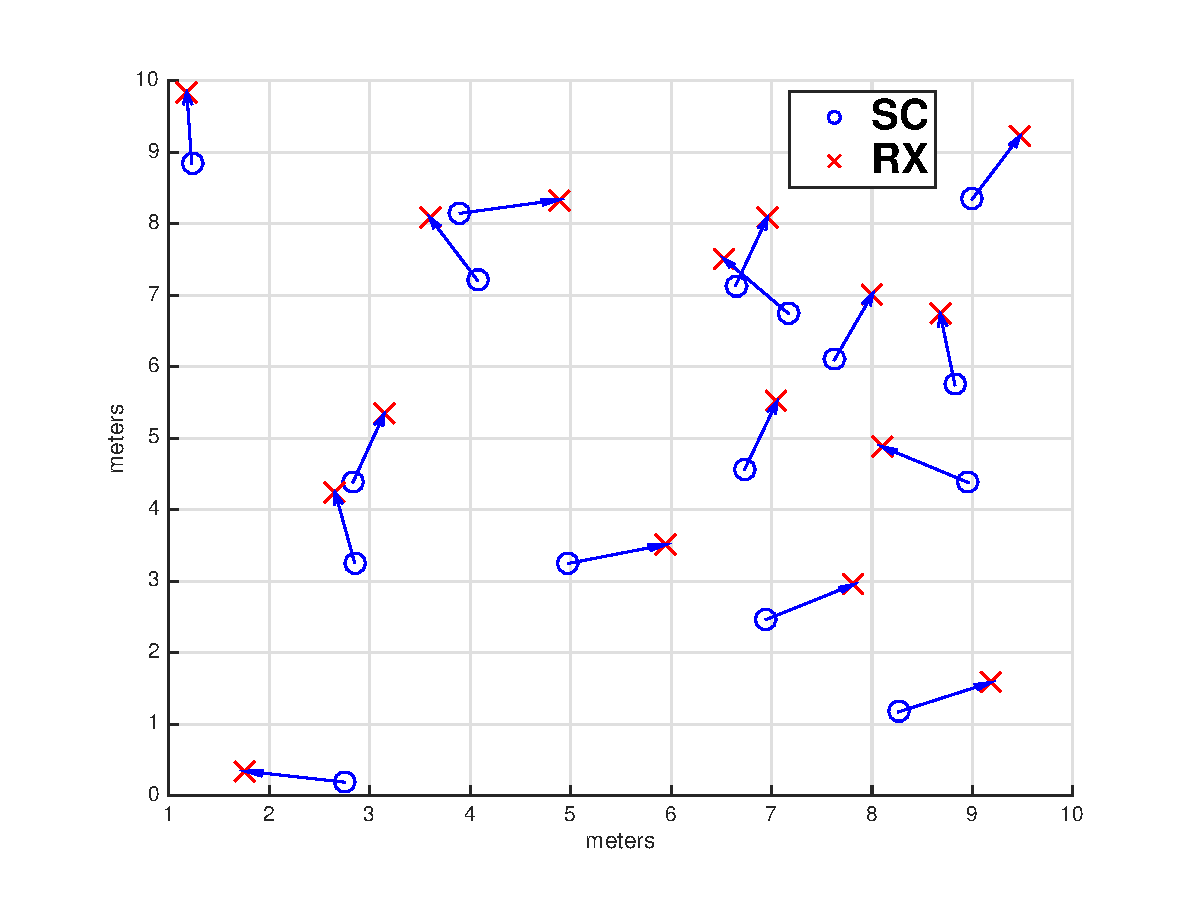
\includegraphics[width=\textwidth]{node_layout.eps}
	\caption{Example realization of PPP network arrangement.}
\end{figure}
%
\subsection{Interference}
%
Now that we have an understanding on the physical placement of nodes in the network we will address the concept of interference.  A common metric used to cellular networks is signal to interference plus noise ratio (SINR).  Assuming constant power $P$ of each network node and noise power $N$, the SINR at each receiver is shown in equation~\eqref{eq:SINR}.
%
\begin{equation}\label{eq:SINR}
  SINR(\textbf{x}_i) = \frac{S}{I(\textbf{x}_i) + N}
\end{equation}
%
$S$ and $I$, the power received from the desired transmitted and combined interferers respectively, are provided in equation~\eqref{eq:Powers}.  $I$ is a SN process, formed by the sum of all spatially random points of $\Phi$.  To remove the path loss singularity around the receiver itself we will assume a minimum distance $\epsilon$ between the receiver and all transmitters.  The channel $h$ is a positive random variable with unit mean.
%
\begin{equation}\label{eq:Powers}
  S = Pl_{\alpha,\epsilon}(u) = Ph_iu^{-\alpha},\quad I(\textbf{x}_i)=\sum_{k\in \Phi,k\neq i} Ph_kl_{\alpha,\epsilon}(|x_i-x_k|)
\end{equation}
%
\todo[inline]{Explain shot noise}
%
\todo[inline]{ADD stuff about performance metrics here}
%
\iffalse % Start comment
%
From SINR we can develop the performance metrics of the network.  We will begin with outage probability $q$.  Outage probability is defined in equation~\eqref{eq:outage} as the probability of SINR values below some threshold $T$.  By extension throughput, which will be discussed in the next section, provides the maximum spatial reuse which is computable by looking at the network at a single snapshot in time.
%
\begin{equation}\label{eq:outage}
  q(\lambda) = P\{SINR<T\}
\end{equation}
%
Expanding~\eqref{eq:outage} further by inserting~\eqref{eq:Powers}
%
\begin{equation}\label{eq:outageMore}
  \begin{split}
  q(\lambda) &= P\Big\{\frac{S}{I + N}<T\Big\}\\
  &= P\Big\{I > \frac{S}{T} - N\Big\} \\
  &= P\Big\{\sum_{k\in \Phi,k\neq i} Ph_kl_{\alpha,\epsilon}(|x_i-x_k|) > \frac{S}{T} - N\Big\}
\end{split}
\end{equation}
%
By the mapping proposition of \cite{Weber2012}, we can rewrite the last equation in \eqref{eq:outageMore} as
%
\begin{equation}\label{eq:outageMapped}
  \begin{split}
  q(\lambda) &= P\Big\{\sum_{k\in \Phi,k\neq i} Ph_kl_{\alpha,\epsilon}(|x_i-x_k|) > \frac{S}{T} - N\Big\} \\
  &= \Big(\frac{\lambda c_d}{2}\Big)^{\alpha/d}\sum_{k\in \Phi,k\neq i}h_i (|x_i-x_k|^{-\alpha})
\end{split}
\end{equation}\todo[size=\small,color=green!50]{Fix}\par
%
RECHEK LAST LINE
%
\subsection{Spatial Capacity}
%
The initial understanding of the network we want to make clear is the spatial capacity of a network given an intensity.  \cite{Weber2012} provides results for the constant transmission case, the slotted aloha case, and the F-Aloha (frequency) case.  This can be considered a circle packing problem, where circle's radius is the range at which the SINR requirement is met.  The transmission capacity is simply equation~\eqref{eq:tc_exact}, with the assumption of no outage probability ($q^*=0$).
%
\begin{equation}\label{eq:tc_exact}
  \lambda(q^*) = \frac{1}{\pi} \sqrt{\frac{ \frac{u^{-4}}{\tau} -\frac{N}{P}}{\pi/2} } F_z^{-1}\Big(\frac{1+q^*}{2}\Big)(1-q^*)
\end{equation}
%
\todo[inline]{Add more}
\section{CSMA}
%
Representation of a CSMA network requires use of the Mat\'ern hard-core PP.  This PP requires a minimum distance $r$ between points, or in our case transmitting nodes.  A Mat\'ern PP is generated from a marked PPP, where each point $x$ uniformly selects a mark $m(x)\in[0,1]$.  Points with marks larger than their neighboring point's marks are deleted if their positions are within range $r$.  Mathematically if $m(x)<m(y)$ and $\|x-y\| \leq r$, point $y$ is deleted.  This is process called conservative, since points that are already deleted can delete other points with larger marks. This is inaccurate in CSMA networks, but it is a common technique in the literature literature~\cite{Nguyen2007}.\par
%
To analyze the intensity of such PP, requires conditioning on existence of points at specific locations.  Palm theory formalizes the notion of the conditional distribution of a PP given it has a point at some location. Note that for a PP without a fixed \textit{atom} at this particular location, the probability of the condition is equal to zero and the basic discrete definition of the conditional probability does not apply~\cite{baccelli2009stochastic}.\par
%
\fi % End comment
